\PassOptionsToPackage{quiet}{fontspec}
\documentclass[12pt,a4paper,UTF8]{article}
\usepackage{thesis} % 格式控制
\usepackage{indentfirst}
\usepackage{amsmath} % 数学公式支持
\usepackage{amsfonts} % 数学字体支持
\usepackage{amssymb} % 数学符号支持
\usepackage{graphicx} % 图片插入支持
\usepackage{float} % 浮动体位置控制，支持 [H] 选项
\usepackage{caption} % 图表标题格式控制
\usepackage{geometry} % 页面布局控制
\usepackage{setspace} % 行距控制
\usepackage{xeCJK} % 中文字体支持
\usepackage{fontspec} % 字体设置
\usepackage[most]{tcolorbox} % 高亮按键命令
\setlength{\parindent}{2em} % 控制首行缩进  
\addtolength{\parskip}{3pt} % 控制段落距离  
\onehalfspacing % 1.5倍行距  
\graphicspath{{./figures/}} % 指定图片所在文件夹  
\setCJKmainfont{SimSun}
% 定义中文字体命令
\setCJKfamilyfont{hei}{SimHei} 

\classname{边缘计算开发实践}  % 设置课程名称
\makepagestyle{}{\printclassname ~实验报告}

% 自定义命令
\newtcbox{\keyblue}{on line,
  colframe=blue!60!black, colback=blue!10,
  boxrule=0.8pt, arc=2pt, boxsep=0pt, left=2pt, right=2pt, top=1pt, bottom=1pt,
  tcbox raise base, fontupper=\color{blue}\bfseries}

\begin{document}
\maketitlepage{盒 驿 卫}{玉泉高分子楼-401}{}{}{\today}{皇甫江涛} %封面页 

\maketoc    %目录页
\section{实物制作}

\subsection{PCB设计}

使用嘉立创EDA进行PCB设计，集成Arduino Nano 33 BLE和ESP8266模块。
整体采用双层板布局，由于考虑到铺铜会影响到WiFi信号，故此处未进行铺铜.

\begin{figure}[H]
    \centering
    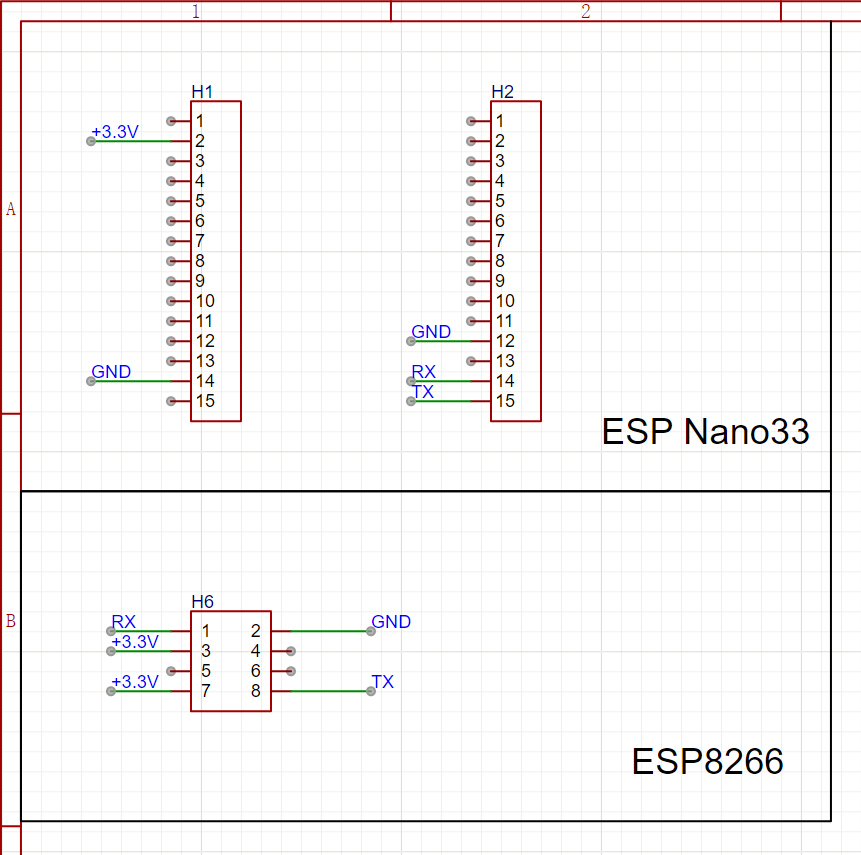
\includegraphics[width=0.7\textwidth]{p1.png}
    \caption{PCB设计原理图}
\end{figure}

\begin{figure}[H]
    \centering
    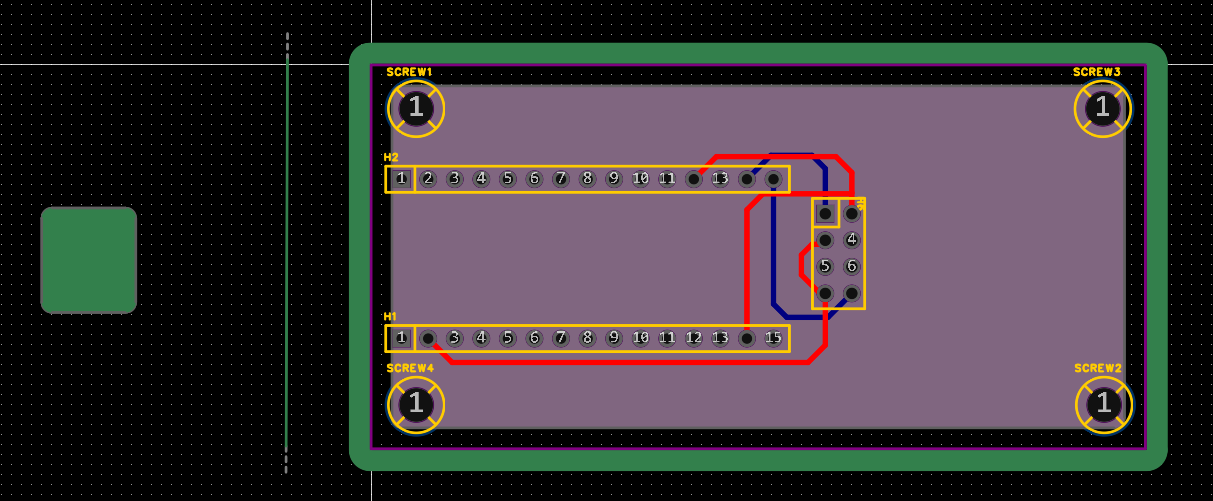
\includegraphics[width=0.8\textwidth]{p2.png}
    \caption{PCB设计布线图}
\end{figure}

\subsection{机械制作}

由于机械模型整体较为简单，此处不考虑使用 solidworks 等专业机械设计工具，而直接在嘉立创中进行设计。

整体采用上下盖分体式设计，预留PCB固定柱和螺丝孔，固定方式选用M3x16沉头自攻螺丝，
侧边开孔位置对应Arduino Nano 33的供电口，
顶上做浅槽开口以嵌入面板。整体使用3D打印制作，
材料使用LEDO 6060 SLA光敏树脂(金属材料可能会屏蔽WiFi信号)。

\begin{figure}[H]
    \centering
    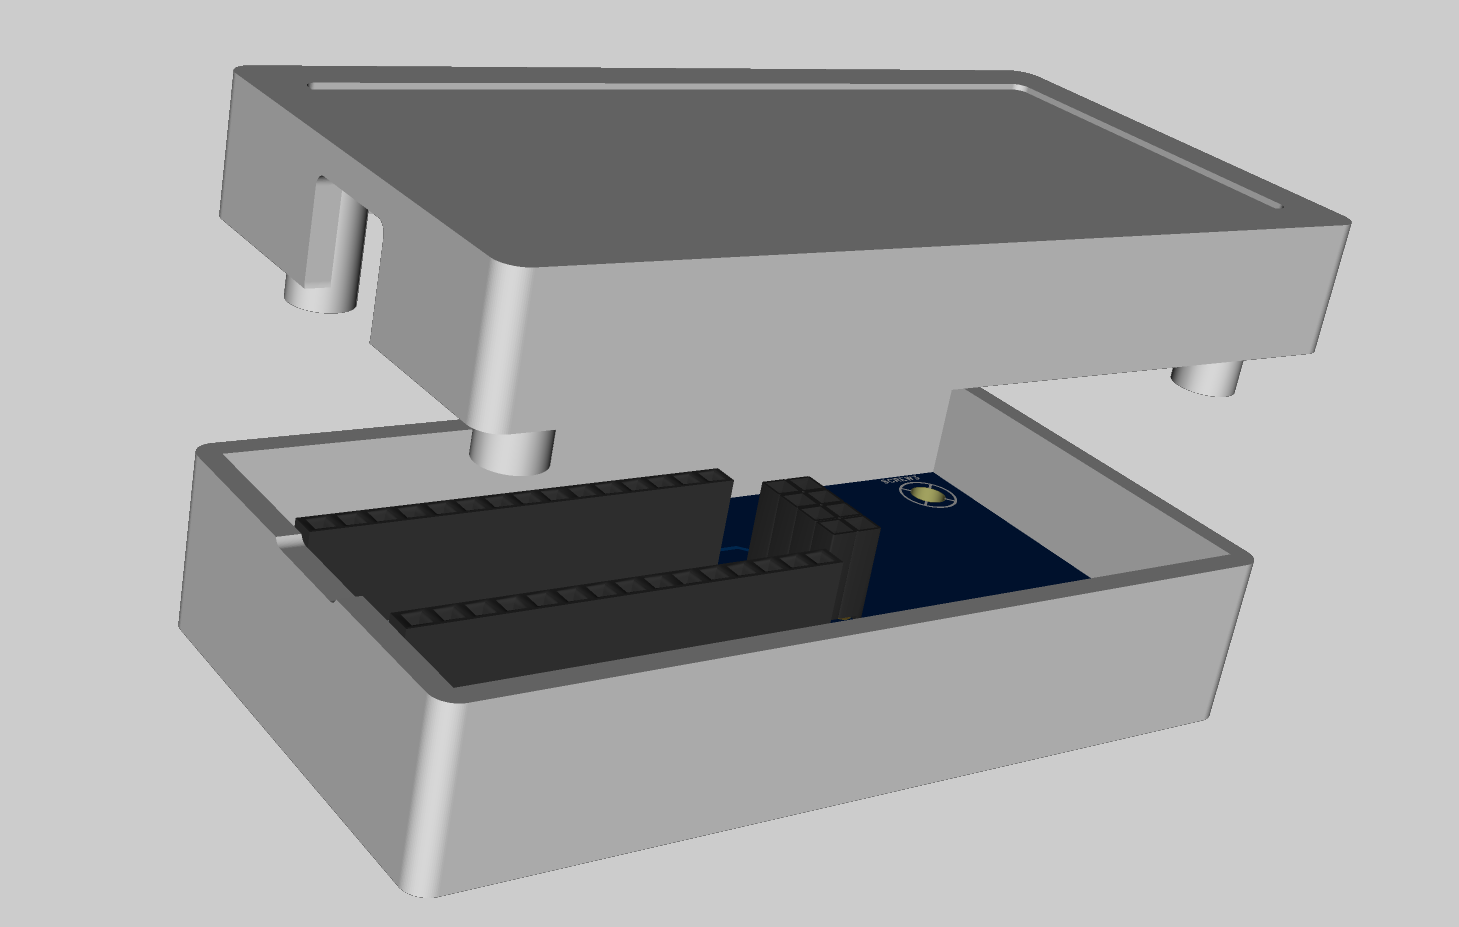
\includegraphics[width=0.8\textwidth]{p3.png}
    \caption{3D外壳设计爆炸图}
\end{figure}

\begin{figure}[H]
    \centering
    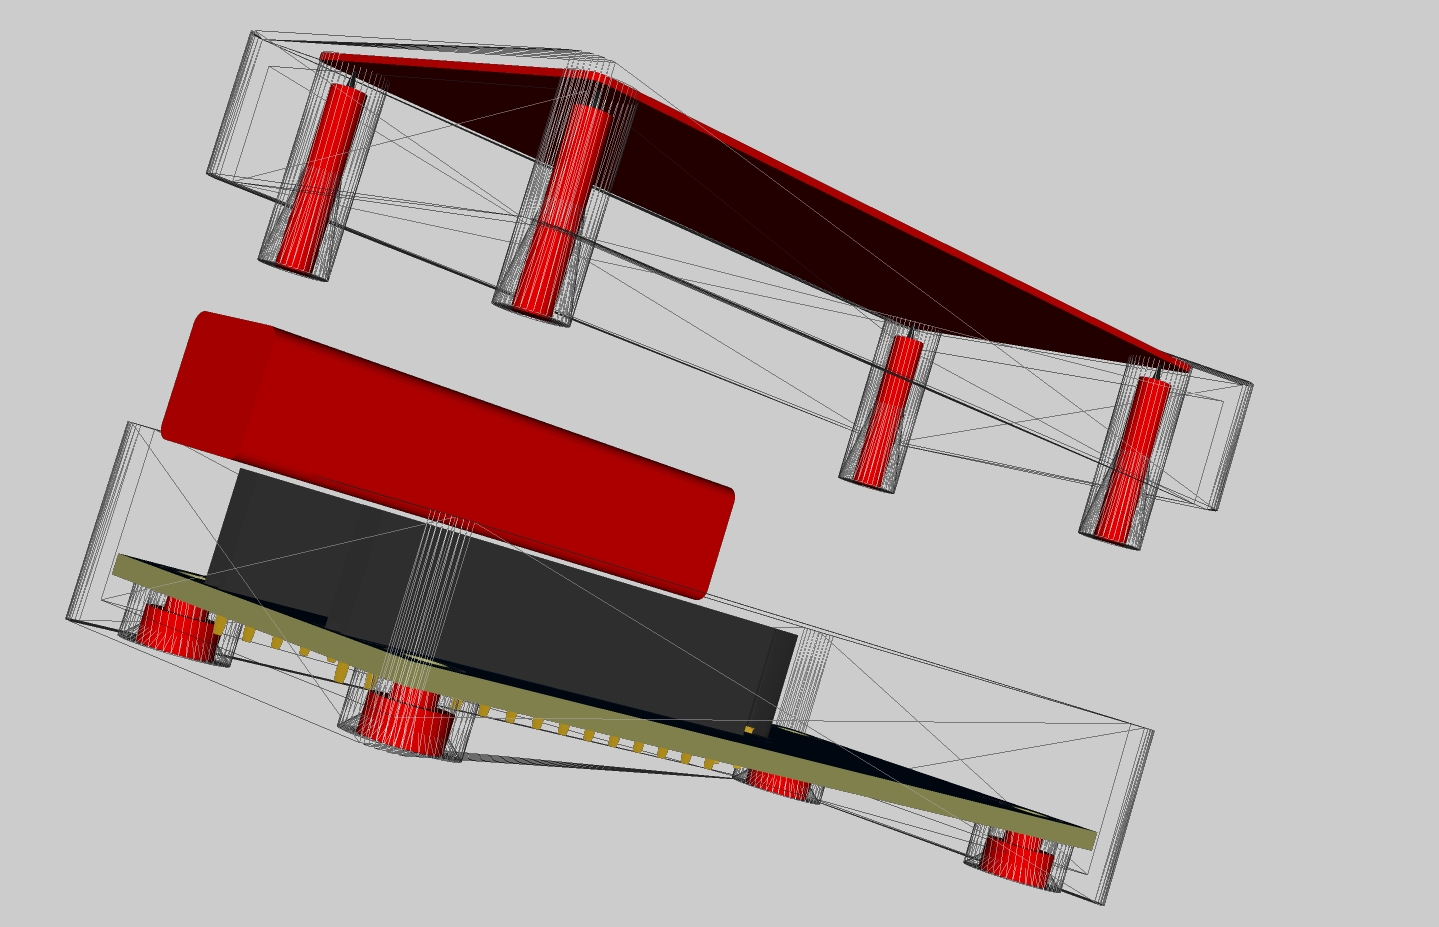
\includegraphics[width=0.8\textwidth]{p4.png}
    \caption{3D外壳设计透视图}
\end{figure}

\subsection{面板制作}

面板采用透明亚克力材质，厚度为浅槽深度0.5mm，通过激光雕刻标注设备名称
，附带信息与电子工程学院ISEE院标。
\begin{figure}[H]
    \centering
    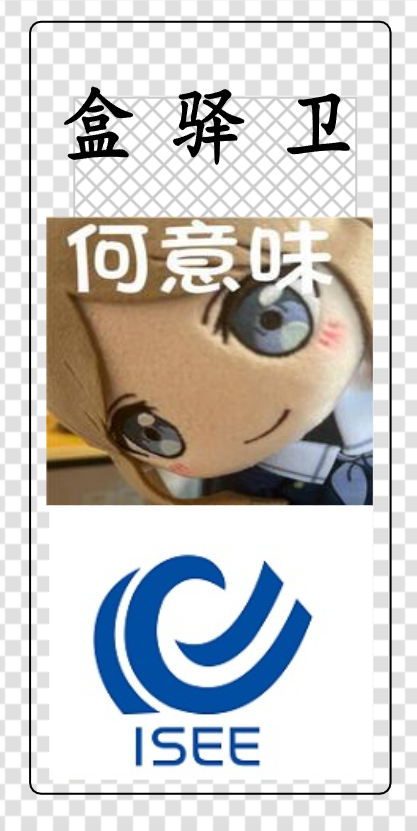
\includegraphics[width=0.2\textwidth]{p5.png}
    \caption{面板设计图}
\end{figure}

\subsection{实物图}

完成PCB焊接和外壳组装，接入Nano33与ESP8266后的成品。如下图：

\begin{figure}[H]
    \centering
    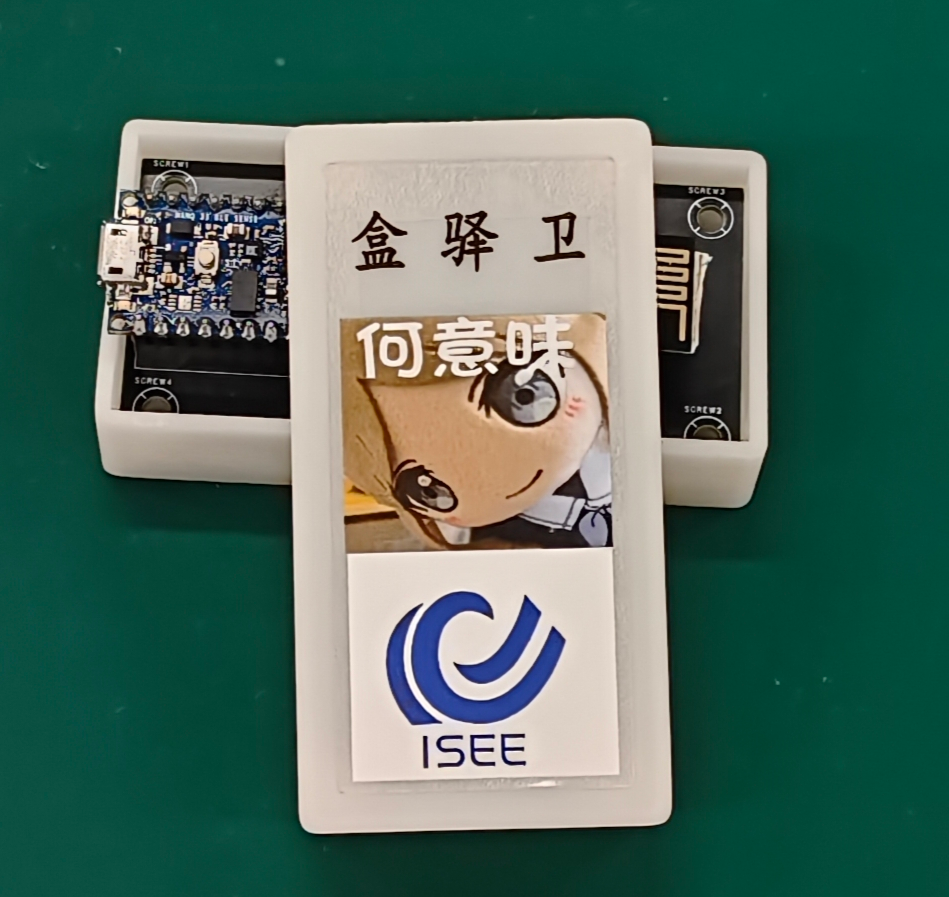
\includegraphics[width=0.6\textwidth]{p6.png}
    \caption{最终实物图}
\end{figure}

\section{遇到问题}

由于设计机械时没有Arduino Nano 33与ESP8266模型，设计时尺寸较难把控，只能在现实中量取并设计，又为了尽可能减小整体体积，保证美观，
导致第一版外壳高度偏低，后续重新设计改正，但第二版仍存在边缘略微错位情况，后续设计时应先保证余量预留充足，再考虑缩减尺寸

\end{document}
